\begin{frame}{Enoncés quantitatifs}
\textbf{Deuxième étape :} formuler une version controlée de la conjecture de Baum-Connes.\\
\vspace{0.3 cm}
Pour cela, il nous faut d'abord introduire les propriétés suivantes :\\
\vspace{0.3 cm}
\begin{itemize}
\item[$\bullet$] $QI_{G,B}(E,E',F,\varepsilon)$ : pour tout $x\in RK^G(P_E(G), B )$, alors $\mu^{\varepsilon,E,F}_{G,B}(x) = 0$ implique que $q_E^{E'}(x)=0$ dans $RK^G(P_{E'}(G),B)$.
\vspace{0.3 cm}
\item[$\bullet$] $QS_{G,B}(E,F,F',\varepsilon,\varepsilon')$ : pour tout $y\in K^{\varepsilon,F}(B\rtimes G)$, il existe $x\in RK^G(P_E(G),B)$ tel que $\mu^{\varepsilon',E,F'}_{G,B}(x)=\iota_{\varepsilon,F}^{\varepsilon',F'}(y)$.\\
\end{itemize} 
\end{frame}

\begin{frame}{Enoncés quantitatifs}
Les énoncés quantitatifs forment le résultat central de la thèse. Ils prennent la forme suivante. Soit $G$ un groupoïde étale $\sigma$-compact à base compacte.\\
\vspace{0.3 cm}
\begin{thmfr}[Injectivité Quantitative]
Soient $B$ une $G$-algèbre, et $\tilde B = l^\infty(\N,B\otimes\mathfrak K)$. Alors 
$\mu_{G,\tilde B}$ est injective ssi 
pour tout $E\in\mathcal E,\varepsilon\in(0,\frac{1}{4})$ et $F$ tel que $k_J(\varepsilon).E\subseteq F$, il existe $E' \in\mathcal E$ tel que $E\subseteq E'$ et $QI_{G,B}(E,E',\varepsilon,F)$ soit vérifiée.
\end{thmfr}
\vspace{0.3 cm}
$\hat\mu_{G,B}$ est quantitativement injective ssi $\mu_{G,\tilde B}$ est injective.
\end{frame}

\begin{frame}{Enoncés quantitatifs}
\begin{thmfr}[Surjectivité Quantitative]
Soient $B$ une $G$-algèbre, et $\tilde B = l^\infty(\N,B\otimes\mathfrak K)$. Alors il existe $\lambda \geq 1$ tel que $\mu_{G,\tilde B}$ est surjective ssi pour tout $0<\varepsilon<\frac{1}{4\lambda}$ et $F\in\mathcal E$, il existe $E\in\mathcal E$ et $F'$ tel que $k_J .E \subseteq F$ tel que $QS_{B,G}(E,F,F',\varepsilon,\lambda\varepsilon)$ soit vérifiée.
\end{thmfr}
\vspace{0.3 cm}
$\hat\mu_{G,B}$ est quantitativement surjective ssi $\mu_{G,\tilde B}$ est surjective.
\end{frame}

\begin{frame}{Enoncés quantitatifs}
Ils admettent une version uniforme :
\begin{thmfr}[Version uniforme] Soit $G$ un groupoïde étale $\sigma$-compact avec une base compacte. \\
\begin{itemize}
\item[$\bullet$] Supposons que pour toute $G$-algèbre $B$, $\mu_{G,B}$ soit injective. Alors, pour tout $\varepsilon\in (0,\frac{1}{4})$ et tout $E,F\in\mathcal E$ tels que $k_J(\varepsilon). E\subseteq F$, il existe $E'\in\mathcal E$ tel que $E\subseteq E'$ et tel que $QI_{G,B}(E,E',\varepsilon,F)$ soit satisfait pout toute $G$-algèbre $B$.\\
\item[$\bullet$] Supposons que pour toute $G$-algèbre $B$, $\mu_{G,B}$ soit surjective. Alors, pour un certain $\lambda \geq 1$ et pour tout $\varepsilon\in (0,\frac{1}{4\lambda})$ et tout $F\in\mathcal E$, il existe $E,F'\in\mathcal E$ tels que $k_J(\varepsilon). E\subseteq F'$ et $F\subseteq F'$ tel que, pour toute $G$-algèbre $B$, $QS_{G,B}(E, F,F',\varepsilon,\lambda \varepsilon)$ soit satisfait.
\end{itemize}
\end{thmfr}
La conjecture de Baum-Connes contrôlée à coefficients et la conjecture de Baum-Connes à coefficients sont équivalentes. 
\end{frame}

\begin{frame}{Enoncés quantitatifs}
\[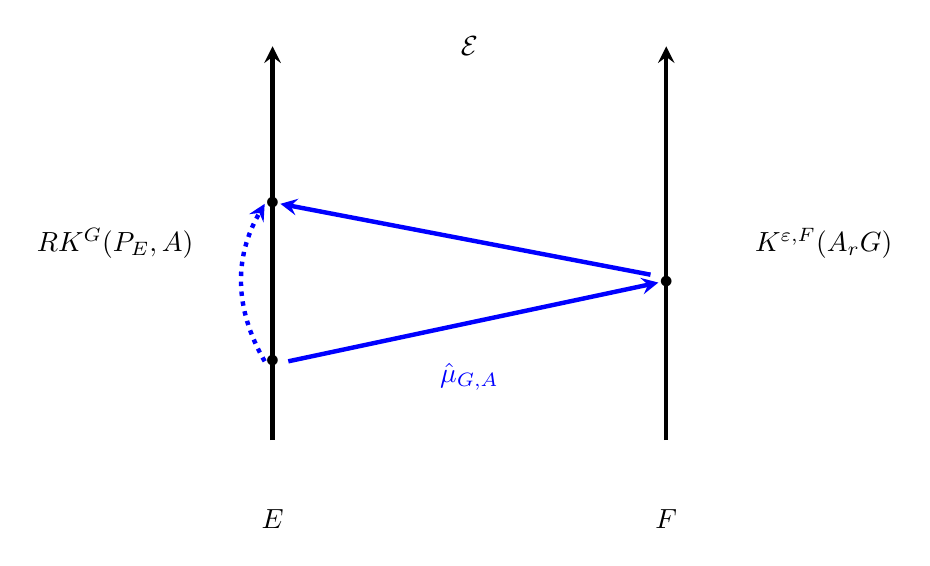
\begin{tikzpicture}
\draw  (2.5,5) node {$\mathcal E$};
\draw  (0,-1) node {$E$};
\draw  (5,-1) node {$F$};
\draw  (-2,2.5) node {$RK^G(P_E,A)$};
\draw  (7,2.5) node {$K^{\varepsilon,F}(A\rtimes_r G)$};
\draw [>=stealth, ->,ultra thick] (0,0) -- (0,5) ; %->
\draw [>=stealth, ->,ultra thick] (5,0) -- (5,5) ; 

\pause
\draw  (0,1) node {$\bullet$};
\draw  (5,2) node {$\bullet$};
\draw [>=stealth, ->,ultra thick, blue] (0.2,1) -- (4.9,2) ; 
\draw[blue] (2.5,0.8) node {$\hat\mu_{G,A}$};

\pause
\draw  (0,3) node {$\bullet$};
\draw [>=stealth, ->,ultra thick, blue] (4.8,2.1) -- (0.1,3) ; 

\pause
\draw [>=stealth, ->,ultra thick, blue, dotted] (-0.1,1) to[bend left] (-0.1,3) ; 

\end{tikzpicture}\]
\end{frame}



















